\documentclass[oneside, 11pt]{article}

\usepackage[T1]{fontenc}
\usepackage[utf8]{inputenc}
\usepackage[dutch]{babel}

\usepackage{fouriernc}
\usepackage[detect-all, load-configurations=binary,
            separate-uncertainty=true, per-mode=symbol,
            retain-explicit-plus, range-phrase={ tot }]{siunitx}

\usepackage{setspace}
\setstretch{1.2}

\setlength{\parskip}{\smallskipamount}
\setlength{\parindent}{0pt}

\usepackage{geometry}
\geometry{marginparwidth=0.5cm, verbose, a4paper, tmargin=3cm, bmargin=3cm, lmargin=2cm, rmargin=2cm}

\usepackage{float}

\usepackage[fleqn]{amsmath}
\numberwithin{equation}{section}
\numberwithin{figure}{section}

\usepackage{graphicx}
\graphicspath{{Figures/}}
\usepackage{subfig}

\usepackage{tikz}
\usetikzlibrary{plotmarks}

\usepackage{fancyhdr}
\pagestyle{fancy}
\fancyhf{}
\rhead{\thepage}
\renewcommand{\footrulewidth}{0pt}
\renewcommand{\headrulewidth}{0pt}

\usepackage{relsize}
\usepackage{xspace}
\usepackage{url}

\newcommand{\figref}[1]{Figuur~\ref{#1}}

\newcommand{\hisparc}{\textsmaller{HiSPARC}\xspace}
\newcommand{\kascade}{\textsmaller{KASCADE}\xspace}
\newcommand{\sapphire}{\textsmaller{SAPPHiRE}\xspace}
\newcommand{\jsparc}{\textsmaller{jSparc}\xspace}
\newcommand{\hdf}{\textsmaller{HDF5}\xspace}
\newcommand{\aires}{\textsmaller{AIRES}\xspace}
\newcommand{\csv}{\textsmaller{CSV}\xspace}
\newcommand{\python}{\textsmaller{PYTHON}\xspace}
\newcommand{\corsika}{\textsmaller{CORSIKA}\xspace}
\newcommand{\labview}{\textsmaller{LabVIEW}\xspace}
\newcommand{\daq}{\textsmaller{DAQ}\xspace}
\newcommand{\adc}{\textsmaller{ADC}\xspace}
\newcommand{\adcs}{\textsmaller{ADC}s\xspace}
\newcommand{\Adcs}{A\textsmaller{DC}s\xspace}
\newcommand{\hi}{\textsc{h i}\xspace}
\newcommand{\hii}{\textsc{h ii}\xspace}
\newcommand{\mip}{\textsmaller{MIP}\xspace}
\newcommand{\hisparcii}{\textsmaller{HiSPARC II}\xspace}
\newcommand{\hisparciii}{\textsmaller{HiSPARC III}\xspace}
\newcommand{\pmt}{\textsmaller{PMT}\xspace}
\newcommand{\pmts}{\textsmaller{PMT}s\xspace}

\DeclareSIUnit{\electronvolt}{\ensuremath{\mathrm{e\!\!\:V}}}

\DeclareSIUnit{\unitsigma}{\ensuremath{\sigma}}
\DeclareSIUnit{\mip}{\textsmaller{MIP}}
\DeclareSIUnit{\adc}{\textsmaller{ADC}}

\DeclareSIUnit{\gauss}{G}
\DeclareSIUnit{\parsec}{pc}
\DeclareSIUnit{\year}{yr}



\title{Weerstation met Arduino}
\author{C.G.N. van Veen}
\docwerkblad{2}{WA}
\version{1.0}

\begin{document}

\maketitle

\section{Weerstation}

\paragraph{Inleiding}
Naast het meten aan kosmische straling met het \hisparc meetstation kunnen  
leerlingen het \hisparc station uitbreiden met een weerstation gemaakt met Arduino.
Dit weerstation heeft als voordeel dat leerlingen dit zelf kunnen bouwen, aanpassen,
programmeren, wind- en water dichtmaken in een box en plaatsen bij het station.
Zo kunnen zij metingen van luchtdruk, buitentemperatuur en temperatuur van de 
detectorplaten meten en correleren met gemeten kosmische straling. Daarnaast 
kan het station uitgebreid worden met andere sensoren zoals UV-index, bliksem, 
regen- en windsensoren.

\begin{figure}
    \centering
    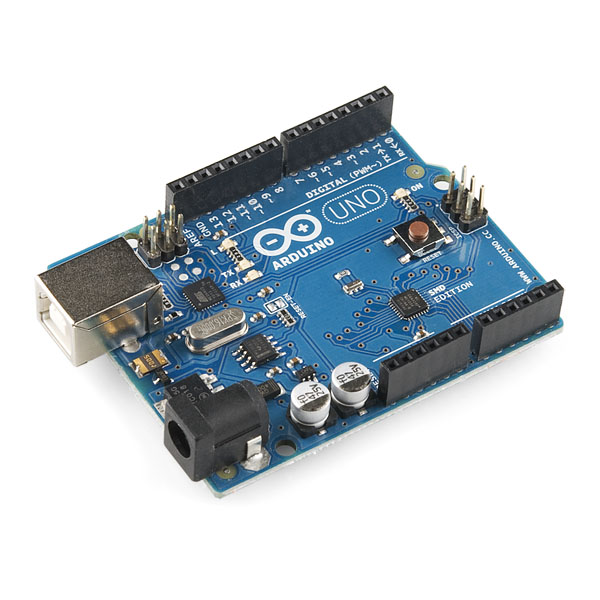
\includegraphics[scale=1.0]{Arduino}
    \caption{Arduino Uno R3, basis voor weerstation}
   \label{fig:Arduino}
\end{figure}

\paragraph{Benodigdheden}
Het weerstation kan met meer sensoren uitgerust worden dan hier genoemd.
Het basis weerstation (luchtdruk, temperatuur en luchtvochtigheid) waar wij mee
getest hebben heeft de volgende onderdelen nodig: \\
\begin{itemize}
    \item Arduino Uno R3 (of elke andere Arduino)
    \item USB kabel
    \item DTH22 (of DTH11) luchtvochtigheid
    \item BMP085 luchtdruksensor
    \item DS18B20 digitale temperatuursensor (2 of 4x)
    \item APC220 zendmodule
    \item arduino software
\end{itemize}

Andere sensoren zoals een bliksemdetector (AS3935) zijn tot op heden niet getest,
maar geven leerlingen een extra onderzoek mogelijkheid(namelijk de correlatie tussen 
bliksem en kosmische straling.)

Op de schets van een bellenvatfoto is te zien, dat bij de botsing van een 
aanstormend pion op een proton, een kaon en een labda ontstaan. Zie 
\figref{fig:bellenvat}.
Zowel het kaon als het labda zijn instabiel.
Zoek met BINAS uit wat de identiteit is van deeltje x en van deeltje y.
\begin{center}
    \rule{\textwidth}{0.3mm}\\
    \rule{\textwidth}{0.3mm}\\
\end{center}


\end{document}
